\documentclass[a4paper,12pt]{article} % Tipo de documento y tamaño de letra.
\usepackage[utf8]{inputenc} % Para que reconozca caracteres especiales como tildes.
\usepackage[spanish, es-nodecimaldot]{babel} % Para definir el idioma y el formato de fechas en español.
\usepackage{amsmath, amssymb} % Paquetes para símbolos y ecuaciones avanzadas (Para hacer una ecuación con un recuadro).
\usepackage{ragged2e} % Para justificar textos.
\usepackage{multicol} % Para crear columnas.
\usepackage{slashed} % Para generar números o variables canceladas (Una línea diagonal sobre el número o variable).
\usepackage{graphicx} % Paquete para poner graficas.
\usepackage{float} % Para poder dejar la imagen en un punto fijo del documento.
\usepackage{longtable} % Para tablas largas.
\usepackage{cancel} % Para hacer cancelaciones en medio de operaciones.
\usepackage{xcolor} % Para el color y esas cosas.
\usepackage{apacite} % Paquete para citas APA.
\usepackage{fancyhdr} % Para personalizar encabezados y pies de página.
\usepackage{geometry} % Para ajustar márgenes.
\usepackage{setspace} % Para ajustar el interlineado.
\usepackage{natbib} % Para manejar las citas y que no queden pegadas y feas :P.
\usepackage{hyperref} % Para que los enlaces funcionen con su URL.
\usepackage[version=4]{mhchem}  % Versión recomendada para mayor funcionalidad.
\usepackage{chemfig} %También para hacer estructuras químicas.
\usepackage{array} % Para mejor control de las columnas.
\usepackage{siunitx} % Para unidades físicas.


\pagestyle{fancy}
\fancyhf{} % Limpia encabezados y pies de página {violeteterminados
\fancyhead[L]{\textbf{BOLETÍN DE PROBLEMAS.}} % Encabezado izquierdo
\fancyhead[R]{\textbf{TERMODINÁMICA.}} % Encabezado derecho
\fancyfoot[C]{\thepage} % Número de página en el centro del pie

\geometry{headheight=12.96115pt, top=1in, bottom=1in, left=1in, right=1in}
\begin{document}


\begin{figure}[H]
	\centering
	
\includegraphics[width=0.5\textwidth]{Unir.jpg}
\end{figure}

\vspace{\baselineskip}

% Ajustamos manualmente todo ;)
\begin{center}
	\textbf{\Large } \\[0.9cm]
	\vspace{\baselineskip}
	\textbf{Liz Ángel Núñez Torres.} \\[0.6cm]
	\textbf{Grado en Física.} \\[0.6cm]
	\textbf{Universidad Internacional de La Rioja.} \\[0.6cm]
	\textbf{26 de Enero 2026.}
\end{center}


\newpage
\tableofcontents

\newpage

\section{Aumento de Entropía.}

\begin{justify}
    Calcular el aumento de entropía de un foco térmico a la temperatura de \(\SI{120}{\degreeCelsius}\) que absorbe \(5,4 \,cal\) de calor.
\end{justify}

\vspace{\baselineskip}


\begin{justify}
    \textbf{Datos:}
\end{justify}

\begin{multicols}{2}
    \begin{itemize}
        \item \( T = \SI{120}{\degreeCelsius} \Rightarrow 393.15 \, \mathrm{K}. \)
        \item \( Q = 5,4 \, \cancel{\mathrm{cal}} \cdot \frac{4.184 \, \mathrm{J}}{1 \, \cancel{\mathrm{cal}}} = 22.60 \, \mathrm{J}.  \)
    \end{itemize}
\end{multicols}

\vspace{\baselineskip}


\subsection{Fórmula Entropía.}
\begin{justify}
    La entropía se define como:
\end{justify}

\[ \triangle S = \frac{Q}{T}. \]

\vspace{\baselineskip}

\begin{justify}
    Como el foco absorbe calor del exterior. \( \mathbf{+ \, Q} \)
\end{justify}

\subsection{Entropía.}

\begin{justify}
    Aplicamos la fórmula de la entropía con los datos obtenidos.
\end{justify}

\[ \triangle S = \frac{22.60 \, \mathrm{J}}{ 393.15 \, \mathrm{K}}. \]

\vspace{\baselineskip}

\[ \textcolor{violet}{\boxed{ \triangle S = 5.78 \times 10^{-2} \, \mathrm{J}/\mathrm{K}. }} \]

\vspace{\baselineskip}

\section{Rendimiento Ciclo de Carnot.}

\begin{justify}
    Calcular el rendimiento de un ciclo de Carnot que funciona entre los focos a las temperaturas de \( \SI{300}{\degreeCelsius} \) y \( \SI{25}{\degreeCelsius} \).
\end{justify}

\vspace{\baselineskip}

\begin{justify}
    \textbf{Datos:}
\end{justify}

\begin{multicols}{2}
    \begin{itemize}
        \item \( T_1 = \SI{300}{\degreeCelsius} \Rightarrow 573.15 \, \mathrm{K}. \)
        \item \( T_2 = \SI{25}{\degreeCelsius} \Rightarrow 298.15 \, \mathrm{K}. \)
    \end{itemize}
\end{multicols}

\subsection{Ciclo de Carnot.}

\begin{justify}
    El rendimiento de Carnot se define como:
\end{justify}

\[ \eta = 1 - \frac{T_f}{T_c}. \]

\vspace{\baselineskip}

\subsection{Rendimiento.}

\begin{justify}
    Donde \( \mathbf{T_f} \) es la temperatura del \textbf{foco frío} y \( \mathbf{T_c} \) es la temperatura del \textbf{foco caliente}.
\end{justify}

\begin{justify}
    Aplicamos la fórmula sustituyendo con los datos obtenidos.
\end{justify}

\[ \eta = 1 - \frac{298.15 \, \cancel{\mathrm{K}}}{573.15 \, \cancel{\mathrm{K}}}. \]

\[ \eta = 1 - 0.52. \]

\vspace{\baselineskip}

\[ \textcolor{violet}{\boxed{ \eta = 48 \% .}} \]

\vspace{\baselineskip}

\section{Ciclo de Carnot Isotermo.}

\begin{justify}
    Calcular el calor absorbido en la primera etapa isoterma del ciclo de Carnot si la temperatura de foco caliente es de \( \SI{200}{\degreeCelsius} \) y un mol del gas ideal se expande hasta triplicar su volumen.
\end{justify}

\begin{justify}
    \textbf{Datos:}
\end{justify}

\begin{multicols}{2}
    \begin{itemize}
        \item \( T_1 = 200 \, \mathrm{K} \Rightarrow 473.15 \, \mathrm{K}. \)
        \item \( n = 1 \, \mathrm{mol}. \)
    \end{itemize}
\end{multicols}

\begin{multicols}{2}
    \begin{itemize}
        \item \( V_2 = 3V_1. \)
        \item \( R = 8.314 \, \mathrm{J}/\mathrm{mol}\mathrm{K}. \)
    \end{itemize}
\end{multicols}

\vspace{\baselineskip}

\subsection{Primera Ley de la Termodinámica.}

\begin{justify}
    De la primera ley de la termodinámica tenemos:
\end{justify}

\[ \triangle U = W - Q. \]

\begin{justify}
    Como tenemos un \textbf{gas ideal} y el proceso es \textbf{isotermo}, la temperatura es constante y no hay variación de energía interna \( \mathbf{\triangle U}\).
\end{justify}

\[ \triangle U = 0. \]

\begin{justify}
    Por este motivo, el calor es igual al trabajo realizado.
\end{justify}

\[ 0 = W - Q \, \, \, \Rightarrow \, \, \, W = Q . \]

\vspace{\baselineskip}

\subsection{Trabajo Isotermo.}

\begin{justify}
    Por lo tanto, sabemos que el trabajo de un gas en expansión isotermo es:
\end{justify}

\[ W = nRT \ln \left( \frac{V_2}{V_1} \right). \]

\begin{justify}
    Sustitumos.
\end{justify}

\[ W = 1 \, \cancel{\mathrm{mol}} \cdot 8.314 \, \mathrm{J} / \cancel{\mathrm{mol}} \cancel{\mathrm{K}} \cdot 473.15 \, \cancel{\mathrm{K}} \cdot \ln \left( 3 \right).  \]

\[ W = 4321 \, \mathrm{J}. \]

\vspace{\baselineskip}

\subsection{Calor Absorbido.}

\begin{justify}
    Como hemos visto antes, el trabajo de expansión es igual al calor absorbido, por lo tanto.
\end{justify}

\[ \textcolor{violet}{\boxed{ Q = 4.32 \, \mathrm{kJ}. }} \]

\vspace{\baselineskip}

\section{Proceso Adiabático.}

\begin{justify}
    En un proceso adiabático un gas a una atmósfera de presión se expande de \( 4.3 \, l \) a \( 10 \, l\). Calcular la presión final. Dato: el coeficiente adiabático es \(^{5/3}\).
\end{justify}

\begin{justify}
    \textbf{Datos:}
\end{justify}

\begin{multicols}{2}
    \begin{itemize}
        \item \( P_1 = 1 \, \mathrm{atm} \Rightarrow 101325 \, \mathrm{Pa}. \)
        \item \( V_1 = 4.3 \, l. \)
    \end{itemize}
\end{multicols}

\begin{multicols}{2}
    \begin{itemize}
        \item \( V_2 = 10 \, l. \)
        \item \( \gamma = \, ^{5/3}. \)
    \end{itemize}
\end{multicols}

\vspace{\baselineskip}

\subsection{Ecuación  de Poisson.}

\begin{justify}
    Como estamos en un proceso \textbf{adiabático} donde no hay tranferencia de calor, definimos la ecuación de Poisson.
\end{justify}

\[ PV^{\gamma} = \mathrm{cte}. \]

\begin{justify}
    Como la presión y el volumen es constante, se cumple que:
\end{justify}

\[ P_1 V_1^{\gamma} = P_2 V_2^{\gamma}. \]

\begin{justify}
    Despejamos la presión final.
\end{justify}

\[ P_2 = P_1 \left( \frac{V_1}{V_2} \right)^{\gamma}. \]

\vspace{\baselineskip}

\subsection{Presión Final.}

\begin{justify}
    Sustitumos por nuestros datos.
\end{justify}

\[ P_2 = 101325 \, \mathrm{Pa} \, \left( \frac{4.3 \, \cancel{\mathrm{l}}}{10 \, \cancel{\mathrm{l}}} \right).  \]

\vspace{\baselineskip}

\[ \textcolor{violet}{\boxed{ P_2 = 24.8 \, \mathrm{kPa}. }} \]

\vspace{\baselineskip}

\section{Variación de Entropía.}

\begin{justify}
    Calcular la variación de entropía de un foco térmico si cede \( 5.6 \, \mathrm{cal} \) de calor a la temperatura de \( \SI{100}{\degreeCelsius} \).
\end{justify}

\vspace{\baselineskip}

\begin{justify}
    \textbf{Datos:}
\end{justify}

\begin{multicols}{2}
    \begin{itemize}
        \item \( T = \SI{100}{\degreeCelsius} \Rightarrow 373.15 \, \mathrm{K}. \)
        \item \( Q = - 5.6 \, \cancel{\mathrm{cal}} \cdot \frac{4.184 \mathrm{J}}{ 1 \cancel{\mathrm{J}}} = 0-23.43 \, \mathrm{J}.  \)
    \end{itemize}
\end{multicols}

\vspace{\baselineskip}

\subsection{Entropía.}

\begin{justify}
    Sabemos que la definición de la entropía es:
\end{justify}

\[ \triangle S = \frac{Q}{T}. \]

\vspace{\baselineskip}

\subsection{Variación de Entropía.}

\begin{justify}
    Como el foco térmico cede calor, esto nos dice que pierde energía térmica, por lo tanto el \textbf{calor es negativo}.
\end{justify}

\[ \triangle S = - \frac{23.43 \, \mathrm{J}}{373.15 \, \mathrm{K}}. \]

\vspace{\baselineskip}

\[ \textcolor{violet}{\boxed{ \triangle S = - \, 6.28 \times 10^{-2} \, \mathrm{J}/\mathrm{K}. }} \]

\section{Trabajo Máquina de Carnot.}

\begin{justify}
    Calcular el trabajo neto de una máquina de Carnot que opera entre las temperaturas \( \SI{500}{\degreeCelsius} \) y \( \SI{10}{\degreeCelsius}\) si en cada ciclo absorbe 5cal de calor del foco caliente.
\end{justify}

\vspace{\baselineskip}

\begin{justify}
    \textbf{Datos:}
\end{justify}

\begin{multicols}{2}
    \begin{itemize}
        \item \( T_1 = \SI{500}{\degreeCelsius} \Rightarrow 773.15 \, \mathrm{K}. \)
        \item \( Q = 5 \, \mathrm{cal} \cdot \frac{4.184 \mathrm{J}}{1 \mathrm{cal}} = 20.92 \mathrm{J}. \)
    \end{itemize}
\end{multicols}

\begin{multicols}{2}
    \begin{itemize}
        \item \( T_2 = \SI{10}{\degreeCelsius} \Rightarrow 283.15 \, \mathrm{K}. \)
    \end{itemize}
\end{multicols}

\vspace{\baselineskip}

\subsection{Ciclo Carnot.}

\begin{justify}
    Como hemos hecho previamente, enunciamos el ciclo de Carnot.
\end{justify}

\[ \eta = 1 - \frac{T_f}{T_c}. \]

\begin{justify}
    Sustitumos por nuestros datos.
\end{justify}

\[ \eta = 1 - \frac{283.15 \, \cancel{\mathrm{K}}}{773.15  \, \cancel{\mathrm{K}. }} \Rightarrow \eta = 1 - 0.366. \]

\vspace{\baselineskip}

\[ \textcolor{brown}{ \boxed{ \eta = 0.634 .} } \]

\vspace{\baselineskip}

\subsection{Trabajo por ciclo.}

\begin{justify}
    El trabajo neto por ciclo se define:
\end{justify}

\[ W = \eta \cdot Q. \]

\vspace{\baselineskip}

\begin{justify}
    Donde \(\mathbf{Q}\) es el calor absorbido, que \textbf{es positivo dado que el calor entra al sistema que realiza el ciclo.}
\end{justify}

\begin{justify}
    Sustitumos con los datos que hemos obtenido anteriormente.
\end{justify}

\[ W = 0.634 \cdot 20.92 \, \mathrm{J}. \]

\vspace{\baselineskip}

\[\textcolor{violet}{\boxed{ W = 13.26 \, \mathrm{J}. }}\]

\vspace{\baselineskip}

\section{Variación de Entropía Gas Ideal.}

\begin{justify}
    Calcular la variación de entropía de \(2,5 \, \mathrm{mol}\) de un gas ideal que experimenta una expansión isoterma de \(4,5 \, \mathrm{l}\) a \(12,6 \, \mathrm{l}\).
\end{justify}

\begin{justify}
    \textbf{Datos:}
\end{justify}

\begin{multicols}{3}
    \begin{itemize}
        \item \( n = 2.5 \, \mathrm{mol}. \)
        \item \( V_1 = 4.5 \, \mathrm{l}. \)
        \item \( V_2 = 12.6 \, \mathrm{l}. \)
    \end{itemize}
\end{multicols}

\vspace{\baselineskip}

\subsection{Entropía Isoterma.}

\begin{justify}
    La variación de entropía para una expansión isotermna de un gas ideal viene definida como:
\end{justify}

\[ \triangle S = nR \ln \left(\frac{V_2}{V_1}\right). \]

\begin{justify}
    Sustituimos por nuestros datos.
\end{justify}

\[ \triangle S = 2.5 \, \cancel{\mathrm{mol}} \cdot 8.314 \mathrm{J}/\cancel{\mathrm{mol}} \mathrm{K} \cdot \ln \left(\frac{12.5 \, \cancel{\mathrm{l}}}{4.5 \, \cancel{\mathrm{l}}}\right). \]

\vspace{\baselineskip}

\[\textcolor{violet}{\boxed{21.4 \, \mathrm{J}/\mathrm{K}}}.\]

\vspace{\baselineskip}

\section{Variación de Entropía.}

\begin{justify}
    Calcular la variación de entropía de un mol de un gas ideal monoatómico en un proceso isostérico cuya temperatura aumenta de \( \SI{30}{\degreeCelsius} \) a \( \SI{60}{\degreeCelsius} \). Datos: \( C_V = 2 \, \mathrm{cal} \, \mathrm{ mol^{-1}} \, \mathrm{K^{-1}}\).
\end{justify}

\begin{justify}
    \textbf{Datos:}
\end{justify}

\begin{multicols}{2}
    \begin{itemize}
        \item \( T_1 = \SI{30}{\degreeCelsius} \Rightarrow 303.15 \, \mathrm{K}. \)
        \item \( T_2 = \SI{60}{\degreeCelsius} \Rightarrow 333.15 \, \mathrm{K}. \)
    \end{itemize}
\end{multicols}

\begin{multicols}{2}
    \begin{itemize}
        \item \( n = 1 \, \mathrm{mol}. \)
        \item \( C_V = 2 \, \cancel{\mathrm{cal}} / \mathrm{mol} \, \mathrm{K} \frac{4.184 \, \mathrm{J}}{1 \, \cancel{\mathrm{cal}}} = 8.368 \, \mathrm{J} / \mathrm{mol} \, \mathrm{K}. \)
    \end{itemize}
\end{multicols}

\vspace{\baselineskip}

\subsection{Entropía en proceso isostérico.}

\begin{justify}
    La variación de entropía a volumen constante para un \textbf{gas ideal} se define:
\end{justify}

\[ \triangle S = nC_v \ln \left( \frac{T_2}{T_1} \right). \]

\vspace{\baselineskip}

\begin{justify}
    Sustituimos.
\end{justify}

\[ \triangle S = 1 \, \cancel{\mathrm{mol}} \cdot 8.368 \, \mathrm{J}/ \cancel{\mathrm{mol}} \, \mathrm{K} \, \ln \left( \frac{333.15 \, \cancel{\mathrm{K}}}{303.15 \, \cancel{\mathrm{K}.}} \right) \]

\vspace{\baselineskip}

\[ \textcolor{violet}{\boxed{ \triangle S = 7.89 \times 10^{-4} \, \mathrm{J}/\mathrm{K} }}. \]

\vspace{\baselineskip}

\section{Temperatura de un Gas.}

\begin{justify}
    La energía de ionización del hidrógeno es de \( 13,6 \, eV \) (electronvoltios). Calcular la temperatura de un gas para que la energía promedio de las partículas fuera igual a la de ionización del hidrógeno. Datos: \( 1 \, eV= 1.603 \times 10^{-19} \mathrm{J}. \)
\end{justify}

\begin{justify}
    \textbf{Datos:}
\end{justify}

\begin{multicols}{2}
    \begin{itemize}
        \item \( E = 13.6 \, \mathrm{eV}. \)
        \item \( K = 1.603 \times 10^{-19} \mathrm{J}/\mathrm{K}. \)
    \end{itemize}
\end{multicols}

\subsection{Energía de Ionización.}

\begin{justify}
    Transformamos en Julios.
\end{justify}

\[ E = 16.6 \, \cancel{\mathrm{eV}} \cdot \frac{1.603 \times 10^{-19} \mathrm{J}}{ 1 \, \cancel{\mathrm{eV}}}. \]

\vspace{\baselineskip}

\[ \textcolor{brown}{ \boxed{ E = 2.18 \times 10^{-18} \mathrm{J}. } } \]

\vspace{\baselineskip}

\subsection{Cinética de la temperatura.}

\begin{justify}
    La teoría cinética de la temperatura se describe:
\end{justify}

\[ E = \frac{1}{2} \, K \, T. \]

\begin{justify}
    Despejamos la temperatura.
\end{justify}

\[ T = \frac{2E}{3K} \]

\vspace{\baselineskip}

\[ T = \frac{2 \cdot  2.18 \times 10^{-18} \, \cancel{ \mathrm{J}} }{3 \cdot 1.603 \times 10^{-19} \cancel{\mathrm{J}} / \mathrm{K}}. \]

\vspace{\baselineskip}

\[ \textcolor{violet}{\boxed{ T = 1.05 \times 10^{-5} \mathrm{K}. }} \]

\section{Energía Promedio.}

\begin{justify}
    Calcular la energía promedio en electronvoltios de las moléculas de un gas ideal monoatómico a la temperatura de \( \SI{1000}{\degreeCelsius} \).
\end{justify}

\begin{justify}
    \textbf{Datos:}
\end{justify}

\begin{multicols}{2}
    \begin{itemize}
        \item \( T = \SI{1000}{\degreeCelsius} \Rightarrow 1273.15 \, \mathrm{K}. \)
        \item \( K = 1.603 \times 10^{-19} \mathrm{J}/\mathrm{K}.  \)
    \end{itemize}
\end{multicols}

\subsection{Cinética de la temperatura.}

\[ E = \frac{3}{2} K \, T. \]

\begin{justify}
    Sustitumos.
\end{justify}

\[ E = \frac{1}{2} \cdot 1.603 \times 10^{-19} \mathrm{J}/\cancel{\mathrm{K}} \cdot 1273.15 \, \cancel{\mathrm{K}}.  \]

\vspace{\baselineskip}

\[ \textcolor{brown}{ \boxed{E = 2.63 \times 10{-20} \, \mathrm{J}. } } \]

\subsection{Energía Electronvoltio.}

\[ E = 2.63 \times 10{-20} \, \cancel{\mathrm{J}} \cdot \frac{1 \, eV}{ 1.603 \times 10^{-19} \cancel{\mathrm{J}}}. \]

\vspace{\baselineskip}

\[\textcolor{violet}{\boxed{ E = 1.64 \times 10^{-1} \, eV. }}\]

\newpage

\section{Revisión.}

\begin{figure}[H]
    \centering
    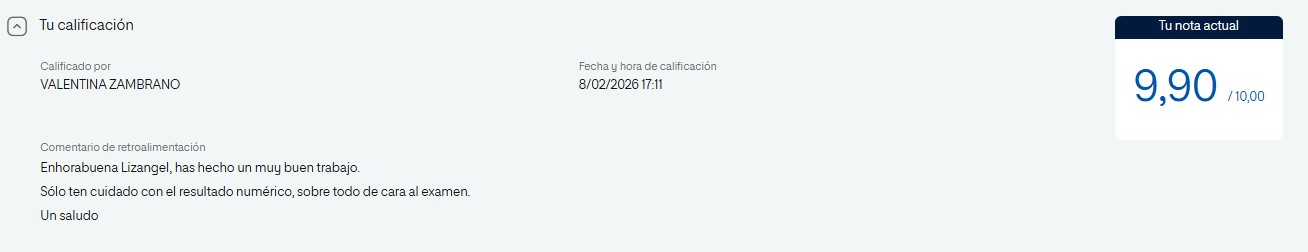
\includegraphics[width=1 \textwidth]{revision.jpg}
\end{figure}




\end{document}